
%
%
% Module: surround_sound_matlab_exercise
%
% Author: Swaroop Appadwedula
%
%

In this section, you will implement the passive
encoder block diagram is shown in Figure \ref{fig:encoder} in \matlab.

\begin{figure}[htb]
    \begin{center}
	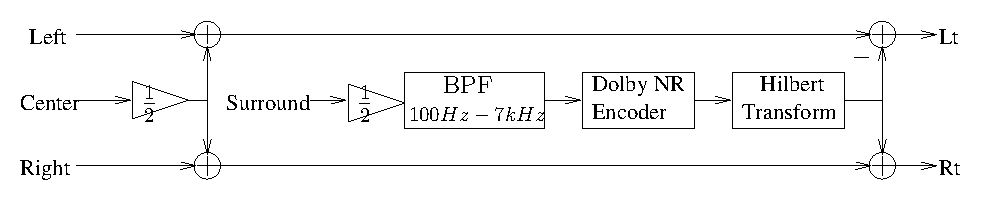
\epsfig{file=encoder.eps,width=13cm}
	\vspace*{0.5cm}
	\caption{Dolby Pro Logic Encoder}
	\label{fig:encoder}
    \end{center}
\end{figure}

The basic components of the encoder are multipliers, adders, a
Hilbert transform, a band-pass filter, and a Dolby Noise
Reduction encoder.  If you wish to implement Dolby Noise
Reduction, refer to \cite{Gundry}.  The other components are
discussed below.

The transfer function of the Hilbert Transform (HT) is shown in Figure
\ref{fig:hilbert}.  The transform is an all-pass filter with
a phase shift of $-90^{o}$.  Observe that a cosine input
becomes a sine and a sine input becomes a -cosine.  In \matlab,
generate a cosine and sine signal of some frequency and use the
\verb+hilbert+ function to do a HT of each signal.  The
imaginary part of the HT output (i.e \verb+imag(hilbert(signal))+)
will be the $-90^{o}$ phase-shifted version of the original signal.
Plot each signal to confirm your expectations.

\begin{figure}[htb]
    \begin{center}
	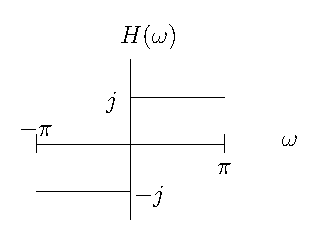
\epsfig{file=hilbert.eps,width=3.0cm}
	\vspace*{0.5cm}
	\caption{Hilbert transform transfer function}
	\label{fig:hilbert}
    \end{center}
\end{figure}

For the bandpass filter, design a second-order Butterworth filter
using the \verb+butter+ function in \matlab.

\paragraph{Generating a surround signal:}  Use simple mixing
techniques to generate a Pro Logic Surround signal.  For example,
use a voice signal for the center channel and fade a roaming sound
such as a helicopter from left to right and front to back.  In
\matlab, use the \verb+wavread+ and \verb+auread+ functions to
read \verb+.wav+ and \verb+.au+ audio files which can be found
on the Internet.


